\section{Results}
\label{sec:results}

In this section, we present results for a set of standard problems in order to validate and evaluate our method. We also compare against classical diffusion (CDA) and flux-limited diffusion (FLD).

Our computer algebra framework and the precomputation has been implemented in Python. The runtime component of our solver has been implemented in C++. We use a naive implementation of a CG solver, which has been modified such that we do not need to expliticly compute the normal form of the linear system to solve. We use the sparse matrix representation and sparse matrix vector product from the Eigen linear algebra library.

The solver for classical diffusion is based on the diffusion equation, which is derived by collapsing the $P_1$-equations:
\begin{align} 
\nabla\left(\frac{1}{3\sigma_t}\nabla L^{0,0}\right)  = -Q^{0,0}
\label{eq:cda}
\end{align}

Since our solver can work with any PDE, which results in a linear system of equations, we put Equation~\ref{eq:cda} into our computer algebra representation and provide it as an input to our solver, which would generate the correct stencil code automatically.

Since FLD is based on a non-linear diffusion equation, we were not able to use our system in the same way. Our implementation closely follows the implementation in~\cite{Koerner14} (though ours runs on CPU) and we refer to their paper for more details.

\subsection{2D checkerboard}

First we ran our solver on the 2D checkerboard, a very common test case in other fields. The problem has dimensions $7\times 7$ and is discretized with resolution $71\times 71$. Unit size blocks are filled with purely absorbing medium with $\sigma_a=10$ in a checkerboard pattern. All other blocks are filled with a purely scattering medium with $\sigma_s=1$.

Solving the standard checkerboard problem, allows us to validate our solver against the solver from Seibold et al.~\cite{Seibold14}, which solves for the time-dependent and complex-valued $P_N$-equations in the 2D case only. The 2D case is derived by assuming that all SH coefficients, RTE parameters and boundary conditions are z-independent. This causes all SH coefficients and moment equations for which $l+m$ is odd to vanish. Due to the time-dependency, their approach is to do explicit incremental steps in time. We run their solver for many timesteps, in order to get a result which is close to steady state.

\begin{figure}[h]
\centering
\begin{subfigure}{0.49\columnwidth}
%\missingfigure{test}
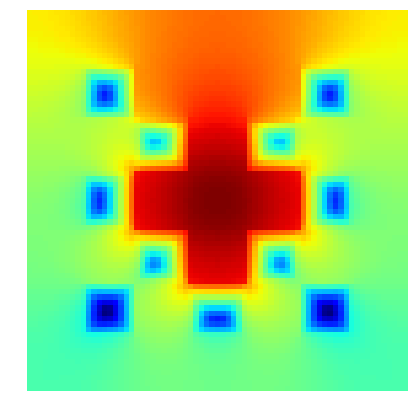
\includegraphics[width=\columnwidth]{images/checkerboard2d_p1_neumann_staggered_starmap.png}
\end{subfigure}%
\hspace{0.01\columnwidth}
\begin{subfigure}{0.49\columnwidth}
%\missingfigure{test2}
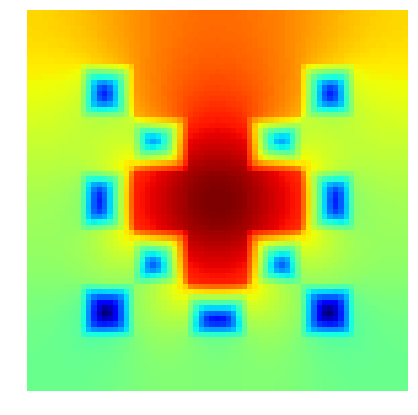
\includegraphics[width=\columnwidth]{images/checkerboard2d_p1_neumann_staggered.png}
\end{subfigure}%
\vspace{-0.2in}
\icaption{Comparison of the result for the checkerboard test using Starmaps time-stepping solver~\cite{Seibold14} (left) against our steady-state solver (right) with $N=5$. Our results are in good agreement.}
\label{fig:vs_starmap}
\end{figure}

As can be seen in figure~\ref{fig:vs_starmap}, the results from our solver are in good agreement with the results from Seibold et al.~\cite{Seibold14} and verify the correctness of our implementation. Converging to a residual of $10e^{-10}$ takes $0.27s$ for $P_1$ and $25s$ for $P_5$.

\subsection{Pointsource problem}

We also run our solver for the point source problem, a single point light in a homogeneous medium. This not only helps to validate our implementation for the 3D case, but also provides information on the accuracy of these methods. We use the Grosjean approximation, which was introduced by D'Eon et al.\cite{dEon11} as a very accurate approximation to the ground truth solution.

\begin{figure}[h]
\centering
\begin{subfigure}{0.45\columnwidth}
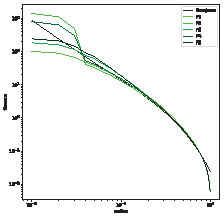
\includegraphics[width=\columnwidth]{figures/pointsource_pn.pdf}
%\missingfigure{test}
\caption{$P_N$ vs. ground truth}
\label{fig:pointsource_pn}
\end{subfigure}%
\hspace{0.05\columnwidth}
\begin{subfigure}{0.45\columnwidth}
%\missingfigure{test2}
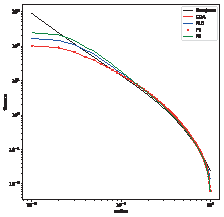
\includegraphics[width=\columnwidth]{figures/pointsource_p5.pdf}
\caption{$P_5$ vs. CDA and FLD}
\label{fig:pointsource_p5}
\end{subfigure}%
\vspace{-0.1in}
\icaption{Lineplot through the 3D solution of our solver for the point source problem for various order $N$ (left). Solution for $P_5$ compared against classical diffusion, flux-limited diffusion and analytical solution (right).}
\label{fig:pointsource}
\end{figure}

For our test case, we choose a FD resolution of $80\times80\times80$, an extinction coefficient $\sigma_t=8.0$ and albedo $\alpha=0.9$. We run the solver for different truncation values $N$. In Figure~\ref{fig:pointsource}~\subref{fig:pointsource_pn}, we see that the solution becomes increasingly accurate for higher truncation order. The ground truth is underestimated when $N$ is odd, and overestimated when $N$ is even. We further see, that the $P_1$ solution exactly matches the results from CDA, which confirmes, that the latter is only a collapsed version of the former. The time to solve is significant with $10m$ for $P_1$ and $45m$ with $P_5$. With these performance characteristics, the $P_N$-method is clearly not competitive in comparison with much diffusion and FLD solver, which are much faster.

\subsection{Nebulae}

Finally, we run our solver on a procedural cloud dataset to get an idea of its performance in more practical applications. Figure~\ref{fig:teaser}~\subref{fig:nebulae_ours} shows the result of $P_5$ for a procedurally generated heterogeneous cloud with an isotropic phase function. We see that at order $N=5$, our method can capture indirect illumination similarily well as FLD and is significantly better than CDA as expected. The indirectly illuminated region at the bottom appears to be closer to the path-traced result as opposed to the solution form FLD which is very flat in that region. However, in many other areas, $P_5$ seems to still suffer a lot from the problem of energy loss near transitions from dense regions to vacuum. It appears that going higher order a few steps, mitigates this problem only slowly at an immense cost of compute and storage.

The main characteristic of the nebulae dataset is the presence of vacuum. We found that having vacuum regions in the dataset will cause the condition number to become infinite and the solver practically doesnt converge. We therefore introduced a minimum threshold for the extinction coefficient $\sigma_t$. Every voxel with an extinction coefficient smaller than the threshold would be set to the threshold value. In Figure~\ref{fig:results_convergence} we show the effect of the minimum threshold on the convergence behavior. As the threshold increases, convergence improves.

%\begin{table}[h]
%\begin{center}
%\begin{tabular}{ c | c c c }
% & \textbf{2D Checkerboard} & \textbf{Point Source} & \textbf{Nebulae} \\ 
%\hline
%$P_1$ & 0.27s & 10m (64\times 64\times 64) & cell6 \\  
%$P_2$ & 2.4s & cell8 & cell9 \\
%$P_3$ & 5.8s & cell8 & cell9 \\
%$P_4$ & 12.7s & cell8 & cell9 \\
%$P_5$ & 25s & ? & ?
%\end{tabular}
%\end{center}
%\icaption{Performance measurements for different datasets and varying truncation order $N$}
%\label{table2}
%\end{table}

\begin{figure}[h]
\centering
%\missingfigure{test}
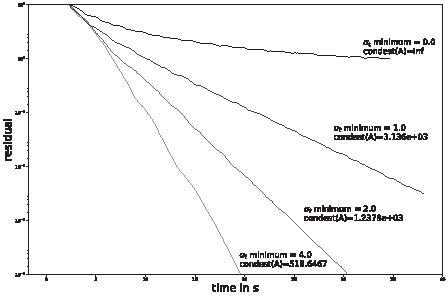
\includegraphics[width=0.9\columnwidth]{figures/fig_nebulae_p1_convergence.pdf}
%\vspace{-0.2in}
\vspace{-0.1in}
\icaption{Convergence behavior of our solver with $N=1$ for the nebulae dataset and for varying minimum thresholds of the extinction coefficient $\sigma_t$. Threshold values and an estimate for the condition number of $A$ (Matlabs condest function) are shown next to the plots. The convergence deteriorates as the threshold decreases. Once it reaches zero, the presence of pure vaccuum makes the condition number infinite.}
\label{fig:results_convergence}
\end{figure}





%\begin{itemize}
%	\item mention performance.
%	\item run for various values of $N$
%	\item convergence behaviour in vacuum. Clearify
%	\item run for anisotropic problem
%\end{itemize}


